\documentclass{article}
\usepackage{graphicx}
\usepackage{amsmath}
\usepackage{amssymb}
\usepackage{tikz}

\title{Cryptography and Number Theory: \\
       Study of Mathematical Principles behind Encryption Algorithms, \\
       Public-key Cryptography, and the Security of Digital Communication}
\author{Badger Code}
\date{\today}

\begin{document}
\maketitle

\section{Introduction}
Cryptography plays a crucial role in securing digital communication and protecting sensitive information. It relies heavily on various mathematical concepts, with number theory being a fundamental pillar. This paper explores the mathematical principles behind encryption algorithms, public-key cryptography, and their role in ensuring the security of digital communication.

\section{Number Theory in Cryptography}
Number theory provides the mathematical foundation for many cryptographic algorithms. Two essential concepts are modular arithmetic and Euler's totient function.

\subsection{Modular Arithmetic}
Modular arithmetic is the study of arithmetic operations involving remainders. For integers $a$ and $b$ with $b > 0$, the modulo operation is represented as $a \bmod b$, and it calculates the remainder when $a$ is divided by $b$.

\begin{center}
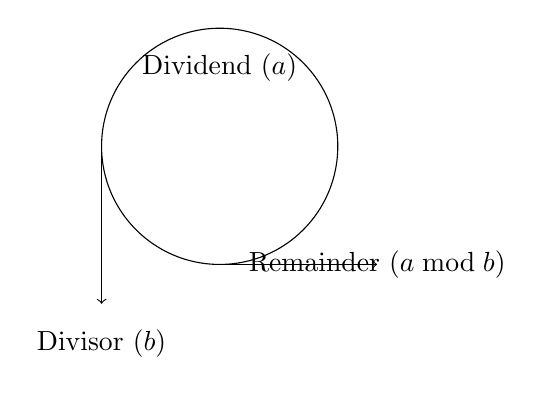
\begin{tikzpicture}
  \draw (0,0) circle (1.5cm);
  \node[align=center] at (0,1) {Dividend ($a$)};
  \draw[->] (-1.5,0) -- (-1.5,-2);
  \node[align=center] at (-1.5,-2.5) {Divisor ($b$)};
  \draw[->] (0,-1.5) -- (2,-1.5);
  \node[align=center] at (2,-1.5) {Remainder ($a \bmod b$)};
\end{tikzpicture}
\end{center}

Modular arithmetic is fundamental in cryptographic algorithms like the Caesar cipher, which is a type of substitution cipher where each letter in the plaintext is shifted by a fixed number of positions down the alphabet.

\subsection{Euler's Totient Function}
Euler's totient function $\phi(n)$ is a crucial concept in number theory and is used in various cryptographic applications. For a positive integer $n$, $\phi(n)$ counts the number of positive integers less than $n$ that are coprime to $n$ (i.e., the numbers whose greatest common divisor with $n$ is 1).

Euler's totient function has significant applications in public-key cryptography, where it is utilized to compute the public and private keys.

\section{Symmetric Encryption Algorithms}
Symmetric encryption algorithms use the same key for both encryption and decryption. They are efficient for encrypting large volumes of data and are commonly used in securing digital communication.

\subsection{Caesar Cipher}
The Caesar cipher is a simple symmetric encryption technique that shifts each letter in the plaintext by a fixed number of positions down the alphabet. For example, with a shift of 3, "A" becomes "D," "B" becomes "E," and so on.

\textbf{Example:} Encrypting the plaintext "HELLO" with a Caesar cipher and a shift of 3 results in the ciphertext "KHOOR."

\subsection{AES (Advanced Encryption Standard)}
AES is a widely used symmetric encryption algorithm. It operates on blocks of data and uses a variable-length key (128, 192, or 256 bits). AES has become the de facto standard for securing sensitive data due to its security and efficiency.

\section{Public-key Cryptography}
Public-key cryptography, also known as asymmetric cryptography, employs a pair of keys: a public key and a private key. The public key is openly distributed, while the private key is kept secret.

\subsection{RSA Algorithm}
The RSA algorithm is a popular public-key cryptosystem invented by Ron Rivest, Adi Shamir, and Leonard Adleman. It relies on the mathematical properties of large prime numbers and Euler's totient function.

The steps of the RSA algorithm include key generation, encryption, and decryption. The security of RSA is based on the difficulty of factoring large composite numbers into their prime factors.

\textbf{Example:} Suppose Alice wants to send a message to Bob using RSA. She encrypts the plaintext message with Bob's public key, and Bob decrypts it with his private key.

\subsection{Diffie-Hellman Key Exchange}
The Diffie-Hellman key exchange is a method for securely exchanging cryptographic keys over an insecure channel. It allows two parties to agree on a shared secret key without directly transmitting it.

The key exchange is based on the difficulty of the discrete logarithm problem. It has various applications, such as establishing a secure communication channel between a client and a server.

\section{Security of Digital Communication}
The mathematical principles of number theory underpin the security of digital communication. By using encryption algorithms and public-key cryptography, sensitive information can be transmitted securely over public networks.

\section{Conclusion}
In conclusion, number theory plays a vital role in modern cryptography. Through modular arithmetic, Euler's totient function, symmetric encryption algorithms, and public-key cryptography, we can ensure the security and privacy of digital communication in an increasingly interconnected world.

\end{document}